\documentclass[10pt]{article}

\usepackage[margin=3cm]{geometry}
\usepackage{amsmath}
\usepackage{amsfonts}
\usepackage{amssymb}
\usepackage{amscd}
\usepackage{standalone}
\usepackage{float}
\usepackage{color}
\usepackage[shortlabels]{enumitem}
\usepackage{graphicx}
\usepackage{caption}
\usepackage[ngerman]{babel}
\usepackage{lscape}
\usepackage{cancel}
\usepackage{dirtytalk}

\graphicspath{ {./images/} }

\begin{document}
\begin{titlepage}
    \centering
    {\scshape\LARGE Hochschule für Technik und Wirtschaft Dresden \par}
    \vspace{1cm}
    {\scshape\Large Softwaresystem \glqq GPS-Track-App\grqq\par}
    \vspace{1.5cm}
    {\huge\bfseries Prjektbericht\par}
    \vspace{2cm}
    {\Large\itshape Raphael Neubert, Alex Schechtel, Aleksandr Pronin, Quang Duy Pham, Tom Nicolai\par}
    \vfill

    {\large \today\par}
\end{titlepage}
\tableofcontents
\newpage
\begin{table}[H]
    \begin{tabular}{lllll}
    \textbf{Vorname} & \textbf{Nachname} & \textbf{Kürzel} &  &  \\
    Aleksandr        & Pronin            & AP              &  &  \\
    Alex             & Schechtel         & AS              &  &  \\
    Quang Duy        & Pham              & QDP             &  &  \\
    Raphael          & Neubert           & RN              &  & 
    \end{tabular}
\end{table}
\section{Projektplanung}
\subsection{Aufgabenstellung [AS]}
    Im Rahmen unserer Projektarbeit im Modul \say{Software Engineering} hat Prof. Mario Neugebauer uns die Möglichkeit gegeben,
    eine Smartphone App zu entwickeln, welche das erstellen von GPS-Tracks für einen mobilen 
    Roboter ermöglicht. Dies hat den Hintergrund, dass die meisten GPS-Tack Apps sehr unflexibel sind und es daher nicht 
    möglich ist, Strecken auf Gegebenheiten des Roboters anzupassen. Das Hauptziel unserer Projektes war es also, eine App zu entwickeln, 
    welche Strecken des Roboters aufnimmt, die er optimal verarbeiten und umsetzen kann.
    Dabei mussten wir für jede implementierte Funktionalität,
    eine angenehme und einfach zu verstehende Darstellungsform für die App finden.
    Es sollte möglich sein die aufgenommenen GPS-Tracks abzuspeichern und in der App aufzulisten.
    Außerdem sollte man auf einem bereitgestellten Server die GPS-Tracks hochladen oder auch herunterladen können.
    Auf den Server sollte jeder Nutzer zugreifen können, welcher eine VPN-Verbindung zu der HTW-Dresden hat.
    Ebenso sollte es die Option geben, die GPS-Tracks nach dem abspeichern noch zu bearbeiten und dabei spezielle Punkte (special points of interests) 
    hinzuzufügen, sowie auch Punkte des aufegnommenen Weges zu verändern/verschieben.
    Bei der Aufnahme eines GPS-Tracks war es außerdem wichtig, die Genauigkeit des GPS-Signals so hoch wie möglich umzusetzen. 
\subsection{Auftraggeber [AP]}
    Die Rolle des Product Owners und Auftraggebers hat Herr Prof. Mario Neugebauer. Die Lehrgebiete von Prof. Neugebauer
    reichen von Programmier- und Datenbankgrundlagen bis hin zu mobilen Systemen und Kommunikationstechnik in 
    mobilen Netzen. Als Product Owner stand er in regelmäßigem Kontakt mit unserem Team, unterstützte uns und
    bewertete die Leistung unseres Teams am Ende der Iteration. Er verfügt über genügend Erfahrung und Wissen,
    um als technischer Ansprechpartner für das Team zu fungieren. Die Zusammenarbeit mit ihm war ein entscheidender Teil 
    unseres Projekts, und sie hat sich als sehr erfolgreich erwiesen.

\subsection{Ausgangssituation [RN], [AS]}
\subsubsection{Softwareengineering-I}
Zu Beginn des Projektes waren wir zu acht. Darunter sechs Informatiker und zwei Wirtschaftsingenieure.
Das Projekt war eine Neuentwicklung. Es gab keinerlei bestehenden Strukturen oder Code. Dies hatte den Vorteil, dass wir
selbst alles Planen konnten und nicht sehr stark an die Entscheidungen von anderen gebunden waren. So konnten wir
selbst die zu verwendenden Technologien, z. B. die Frameworks und Programmiersprachen festlegen und mussten dabei
nur auf die Wünsche des Themenstellers achten. Dies machte es uns natürlich nicht nur leichter, denn auch
hier galt \say{With great power comes great responsibility.}. Wir mussten also sehr viel Zeit in Recherche stecken um
feststellen zu können, ob mit den, von uns ausgewählten Technologien die Funktionalitäten überhaupt implementierbar sind.\par
\medskip
Am Anfang des Projektes fehlte uns vor allem eines, Erfahrung. Erfahrung sowohl in der Verwendung der Technologien
aber viel mehr noch, Erfahrung in der Teamarbeit und der Organisation eines solchen Softwareprojektes.
Dies wurde uns vor allem am Ende von Softwareengineering-I klar, als wir das nochmal Abgabedokument durchschauten
und feststellten, wie ineffizient unsere Arbeit am Anfang war.

\subsubsection{Softwareengineering-II}
Am Ende des Moduls SE1 hatten wir einen guten umfassenden
Überblick in das System und den funktionalen Anforderungen gewonnen. 
Wir hatten jetzt auch schon den Code vom Prototyp. Viel wichtiger aber, wir hatten die Erfahrung und das Wissen, was
wir beides bei der Erstellung des Prototyps erlangt hatten. Somit war der Start in Softwareengineering-II wesentlich
angenehmer als der in Softwareengineering-I.\par
\medskip
Die zwei Mitglieder aus dem Studiengang Wirtschaftsingenieurwesen, verabschiedeten 
sich am Ende des SE1 Projektes.
Außerdem verließ ein weiteres Mitglied die Gruppe. Somit verkleinerte sich unsere Gruppe von acht Mitgliedern,
auf fünf. Jedoch bekamen wir aufgrund unserer geringen Kapazität, 
gegenüber anderen Gruppen ein Ersatzmitglied (Aleksandr Pronin). \par 
\medskip
 Die gute Note, die die Wirtschaftsingenieure erhalten hatten, gab auch den
Rest des Teams viel Motivation und so starteten wir in das Modul mit dem Vorsatz schon am Anfang des Semesters möglichst
viel fertig zu bekommen, um Stress am Ende wenn noch andere Belegarbeiten dazukommen zu vermeiden.
Im ersten Meeting brachten wir alle Mitglieder nochmal auf den selben Informationsstand, 
über die Aufgabenstellung und den Fortschritt. 
Außerdem überprüften wir unsere grobe Rollenverteilung und verteilten die Aufgabenbereiche 
(Server u. App implementierung, Analyst, Tester etc.)
auf die Mitglieder auf. Somit hatten wir alle Voraussetzungen für einen guten Start in das laufende Projekt in SE2.


\subsection{Rollenverteilung [AP], [RN]}
    Die Rollen im Team waren nicht streng verteilt. Jeder war in seinem Bereich und entsprechend seinen Kompetenzen an 
    dem Projekt beteiligt. Im Verlaufe des Projektes entstand von alleine eine Art Zuordnung von Fachgebiet und Person.
    Zum Beispiel war am Ende Alexandr Pronin für die Entwicklung und technischen Lösungen für den Client-Server-Teil verantwortlich 
    und Alex Schechtel für UI-relevante Dinge zuständig. Die folgenden Tabellen zeigen die, zu Beginn der jeweiligen Semester,
    ursprünglichen Rollenverteilungen.
\begin{table}[H]
    \begin{tabular}{|l|l|}
    \hline
    Anton  Peschel    & Projektleitung                                      \\ \hline
    Felix Reuß        & Analyst, Unterstützung Projektleitung               \\ \hline
    Ludwig Schönthier & Analyst,  Test                                      \\ \hline
    Richard Michel    & Any Role                                            \\ \hline
    Raphael Neubert   & Developer, Entwurf, stellvertretende Projektleitung \\ \hline
    Alex Schechtel    & Developer, Tester, Any Role                         \\ \hline
    Tom Nicolai       & Developer, Tester                                   \\ \hline
    Quang Duy Pham    & Tester, Entwurf                                     \\ \hline
    \end{tabular}
    \centering
    \caption{ursprüngliche Rollenverteilung Softwareengineering-I}
\end{table}
\begin{table}[H]
    \begin{tabular}{|l|l|}
    \hline
    Ludwig Schönthier & Analyst,  Projektleitung                                \\ \hline
    Raphael Neubert   & Projektleitung, Developer, Entwurf, Deployment Engineer \\ \hline
    Aleksandr Pronin  & Developer, Entwurf, Deployment Engineer                 \\ \hline
    Alex Schechtel    & Developer,  Any Role                                    \\ \hline
    Tom Nicolai       & Developer, Any Role                                     \\ \hline
    Quang Duy Pham    & Tester, Any Role                                        \\ \hline
    \end{tabular}
    \centering
    \caption{ursprüngliche Rollenverteilung Softwareengineering-II}
\end{table}
Wie in Tabelle 2 zu erkennen ist übernahmen in Softwareengineering-II Ludwig Schönthier und Raphael Neubert die 
Projektleitung. Damit dies möglich war, wurden die Projektleiteraufgaben zwischen den beiden aufgeteilt und auf eine 
ständige Kommunikation in der Projektleitung gesetzt.
\newpage
\subsection{Kommunikation [RN]}
Durch die Pandemie bedingten Einschränkungen haben wir in \say{Softwareengineering-I} ausschließlich online kommuniziert. Später, in \say{Softwareengineering-II} war dies nicht mehr nötig. Da unser Team aus drei verschiedenen
Studiengängen und verschiedenen Jahrgängen bestand, war es durch die verschiedenen Stundenpläne und Nebenjobs 
schwer einen Termin zu finden an dem alle an der HTW sind bzw. an die HTW kommen konnten. Da die online Kommunikation 
schon bei Softwareengineering-I sehr gut funktionierte, entschlossen wir uns bei Softwareengineering-II weiterhin online 
zu kommunizieren.\par
\medskip
Für die online-Kommunikation im Team verwendeten wir die Dienst \say{Element}. Element ähnelt vom Grundaufbau dem 
Dienst \say{Discord}, unterscheidet sich aber insofern, als das Element Open-Source und dezentralisiert ist.
In unserem Element-\say{Space} erstellten wir uns zunächst zwei Kanäle. Einen für allgemeine Besprechungen, 
einen für  Programmierungs- bzw. Implementierungsspezifische Konversationen. Später im Projekt merkten wir, das 
es oft vorkam, das wichtige Informationen im Chat in unwichtigere Informationen untergingen. Wir erstellten
daher noch einen dritten Kanal für alle wichtigen links und Termine.
Für die Meetings verwendeten wir zunächst die von Element bereitgestellte Gruppenanrufs-Funktion.
Nach einigen Updates von Element gab es allerdings einige Probleme bei den Gruppenanrufen. Wir entschlossen 
uns daher von nun an für unsere Meetings die Plattform \say{Jitsi} zu verwenden.
Jitsi ist eine Open-Source Konferenzservice mit dem man im Browser, 
ohne Anmeldung mit zwei Klicks eine Konferenz starten kann. Unsere Erfahrungen mit Jitsi waren ausschließlich positiv.\par
\medskip
Um eine stetige Kommunikation zu gewährleisten und somit die Chance für das Eintreten bzw. die Folgen
von fehlerhafte Kommunikation zu minimieren, trafen wir uns am Anfang des Projektes wöchentlich. Am Ende 
des Projektes war unsere Aufgabenverteilung und unser gegenseitiges Vertrauen gut genug, sodass wir, solange
eine stetige Kommunikation auch asynchron gewährleistet war, zwischen Meetings auch mal zwei Wochen Platz lassen konnten.\par
\medskip
Während unsere Meetings zunächst sehr unkoordiniert abliefen, ergab sich mit der Zeit eine immer besser werdende 
Meetingstruktur. Anfangs haben wir für jedes Meeting sehr aufwändige Protokolle geschrieben. Nach einer Weile stellten 
wir fest das kaum jemand die Protokolle las und uns daher keinen Mehrwert gab. Um einen Ausgleich zwischen 
investierter Zeit und Mehrwert zu bekommen, entschieden wir uns, nur noch die Treffen mit dem Themensteller oder dem Coach
zu protokollieren und in dem Fall, dass jemand an einem Meeting nicht teilnehmen kann, wir uns im Nachhinein mit der 
Person in Verbindung setzen und ihr kurz das Meeting zusammenfassen. Eine weitere Verbesserung erzielten wir dadurch
das wir anfingen das jeder am Anfang des Meetings kurz zeigte, was er in der letzten Zeit gemacht hatte.
Dies wirkte sich auf den allgemeinen Überblick des Teams, aber auch auf die Motivation der einzelnen Personen positiv aus.
Es gab noch kleine weitere Änderungen, die sich positiv auf die Meetings ausgewirkt haben. Neben den 
durch Änderungen ausgelösten diskreten Verbesserungen war aber auch eine, durch den Zuwachs an allgemeiner 
Erfahrung und Kompetenz ausgelöste stetige Verbesserung bemerkbar. Die Früchte der Verbesserungen waren unter anderen 
ein besseren Überblick den jedes Teammitglied über das Projekt hatte, jeder wusste nach dem Meeting genau, was er 
zu erledigen hatte, die Meeting Zeit wurde effizienter genutzt so das in weniger Zeit
mehr Informationen ausgetauscht werden konnten.
\par
\medskip

Am Ende unterteilten sich die Meetings meistens in vier Teile. Als Erstes haben wir immer über die in Ergebnisse
seit dem letzten Meeting gesprochen. Wie bereits erwähnt geschah dies oft so, das die einzelnen Teilnehmer 
kurz ihre fortschritte erklärten bzw. vorführten.  Danach besprachen wir die grobe weitere Planung. Dazu zählte die 
Überprüfung ob wir uns im Zeitplan befinden, die Priorisierung bzw. das Umpriorisieren von Funktionalitäten und die 
Planung von Meetings mit dem Themensteller oder Coach. Als Drittes setzten wir die Planung der aktuellen Funktionalitäten 
fort und erstellten Issues für die Weiterentwicklung. Im letzten Teil des Meetings teilten wir dann die Issues 
den Teammitgliedern zu. Dabei konnte es auch vorkommen, dass wir niedrig priorisierte Issues niemanden zuteilten, sondern 
diese, falls jemand schon schneller als erwartet mit seinen Issues fertig war, dieser Person zugewiesen wurde.\par
\medskip
Um Zeitverschwendung zu vermeiden planten wir die Meetings mit dem Themensteller oder dem Coach nur nach Bedarf.
Wir schrieben uns unsere fragen immer auf und sobald genug zusammengekommen waren bzw. eine Frage sehr 
wichtig war, planten wir ein Meeting. Für die Besprechung von kleinen, wichtigen Entscheidungen,
die schnell getroffen werden mussten war oft auch eine kurze Mail an den Themensteller ausreichend.
Während wir bei Softwareengineering-I häufig Meetings mit unserem Coach hatten, reduzierte sich die Anzahl
bei Softwareengineering-II stark. Dies war vor allem der Tatsache geschuldet das wir uns mehr auf die Entwicklung
der eigentlichen Software konzentrierten aber auch der Tatsache das wir
in unserem arbeiten viel sicherer geworden sind und dadurch weniger Fragen auftraten.
Die Meetings sowohl mit dem Themensteller als auch mit dem Coach empfanden wir immer als sehr sinnvoll. Meist 
trafen wir uns direkt nach dem Meeting, um die vorgeschlagenen dinge in Issues zu überführen die wir dann später 
umsetzten.\par 
\medskip 
Perfekt waren unsere Meetings am Ende aber noch lange nicht. Ein Problem was wir zum Beispiel nur vermindern aber 
noch nicht komplett lösen konnten war das, sich im Meeting beschränken auf Konversationen, die möglichst alle betreffen.
Zum Beispiel haben wir manchmal sehr detailliert über die Serversynchronisation gesprochen und das, obwohl an der 
Entwicklung der Synchronisation nur zwei Personen beteiligt waren. Solche Situationen entstanden unbewusst und 
wirkte sich, für alle am detaillierten Thema unbeteiligten negativ auf die Qualität des Meetings aus.

\subsection{Techniken/Praktiken [RN]}
%hier kann unsere Github nutzung hin. Also projektboard, branches und so weiter.
% vielleicht auch wie wir iterationen planen und wann wir einen neue starten.
\subsubsection{Git/GitHub}
Zur Entwicklung verwendeten wir Git und als Host GitHub. In unserem Team kannten sich anfangs nur zwei von acht Personen
mit Git aus. Wir passten daher die Komplexität unseres GitHub-Workflows dem stand der Praktika an. Zum Beispiel 
verwendeten wir erst mehrere Branches nachdem Branching im Praktikum behandelt wurden. Unsere GitHub-Workflows haben
wir im Verlauf des Projektes sehr häufig angepasst und verbessert.\par
\medskip
Von Anfang an verwendeten wir Issues zur Planung kleiner Aufgaben. Nach einer weile merkten wir das es sinnvoll
ist diese mittels eines Projektboards zu organisieren. Wir erstellten daraufhin ein Projektboard mit vier Spalten.
Die Spalte \say{Icebox} für Issues die noch niemanden Zugewiesen wurden, die Spalte \say{Assigned} für Issues die 
zwar zugewiesen, aber noch nicht in Bearbeitung waren, die Spalte \say{In Progress} für Issues die sowohl zugewiesen 
als auch in Bearbeitung sind, und die Spalte \say{Done} für Issues deren Bearbeitung abgeschlossen ist.
Wir verwendeten dieses Projektboard für mehrere Iterationen. Nachdem es aber immer voller wurde, entschlossen wir uns 
von nun an für jede Iteration ein Projektboard zu erstellen. Im Verlaufe des Projektes versuchten wir uns auch mal 
an der Verwendung eines komplizierteren Projektboards mit Pull-Requests und Reviews, merkten aber schnell, dass 
für den Umfang unseres Projektes, mit dieser Methode, Zeit und Nutzen in keinem guten Verhältnis standen.
Wir können uns allerdings vorstellen das die Verwendung eines solchen Projektboards für Umfangreichere Projekte 
sinnvoll ist. Am ende verwendeten wir primitive 3 Spalten Projektboards mit den Spalten \say{To do}, \say{Assigned} und
\say{Done}, da wir feststellten das wir von der Spalte \say{In Progress} keinen Mehrwert erhielten und es aufwendig 
war, jedesmal bevor man mit der Arbeit anfangen konnte eine Änderung am Board vornehmen zu müssen. Die Projektboards 
automatisierten wir so, dass beim schließen eines Issues, sei es manuell oder durch Referenzierung des Issues in 
der Commit-message, dieser Automatisch in die Spalte \say{Done} verschoben wurde.\par 
\medskip
Wie bereits erwähnt verwendeten wir zunächst nur einen Branch. Für alles was nur mit Dokumentation und Anforderungsanalyse 
zu tun hatte, funktionierte dies Problemlos. Bei der Entwicklung hingegen, gab es ab und zu kleine Probleme.
Zum Beispiel ist es mal vorgekommen das wir festellen mussten, dass kurz vor einem Meeting mit dem Themensteller 
die App nicht mehr Kompilierte. Gelöst haben wir das Problem in dem wir einen \say{checkout} zu einer älteren Version 
gemacht haben und nach dem Meeting den Fehler gesucht und gelöst haben, aber dies brachte uns auf eine Idee.
Wir wollten von nun an mehrere Branches verwenden und für diese, sowie deren Interaktion verschiedene Regeln aufstellen.
Eine Regel war zum Beispiel, dass die sich auf dem Hauptbranch befindende Version immer erfolgreich kompilieren
und keine größeren Bugs beinhalten muss. Wir erstellten den Branch \say{dev} auf dem wir von nun an entwickelten.
Immer wenn eine Funktionalität fertig entwickelt und ausreichen gut getestet war, haben wir den \say{dev}-Branch in 
unseren Hauptbranch gemerged und somit den Hauptbranch aktualisiert. Später versuchten wir für jedes Feature einen 
eigenen Branch zu erstellen und nach fertigstellung diesen in den \say{dev}-Branch zu mergen. Wir mussten aber feststellen 
das dies zum einen sehr aufwendig war, oft aber auch kaum möglich, da es Abhängigkeiten zwischen den Features gab,
die erst bei der Entwicklung auffielen. Wir entschlossen uns daher nur für große, ganz klar unabhängige Features 
weitere Branches zu erstellen und behielten dieses Branching-Modell bis zum Ende des Projektes bei.

\subsubsection{Iterationen}


\section{Projektdurchführung}
\subsection{Iterationsphasen}
\subsubsection{Phase: Inception}
Iteration 1
\subsubsection{Phase: Elaboration}
Iteration 2, 3, 4, 5
\subsubsection{Phase: Construction}
Iteration 6, 7
\subsubsection{Phase: Transition}
Iteration 8
    In dieser Phase sollte realisiert werden, dass das System vom Kunden nutzbar ist. Da die volle Funktionalität bereits in der Phase "Transition" sichergestellt wurde,
    geht es hier ausschließlich um die Dokumentation des Projektes. Die wichtigsten Dokumente stellen dabei die Betriebsanleitung sowie die Nutzeranleitung dar, da diese
    dem Kunden eine vollständige Anleitung der Einrichtung und Bedienung der App sowie des Servers liefern. Zu Beginn der Phase wurde der Fokus auf das Abnahmegespräch
    (24.06.2022) mit unserem Themensteller Prof. Dr. Mario Neugebauer gelegt. Es wurden noch minimale Fixes und Erweiterungen zur Verbesserung des Nutzererlebnisses
    an der App vorgenommen, um eine möglichst reibungsfreie Präsentation unseres Endproduktes zu gewährleisten. Das Abnahmegespräch lief dann auch reibungslos ab. Im
    Anschluss setzten wir uns an die Vervollständigung aller verbleibender Dokumente. Dazu gehörten beispielsweise ein aktualisiertes Abnahmeprotokoll, da das vorherige
    Fehler aufwies oder die Aktualisierung der Screenshots der Risikoliste. Am 04.07.2022 fand die Softwarepräsentation während der Lehrveranstaltung Software Engineering
    statt, in der Raphael und Ludwig den finalen Stand der Software zusammen mit den erreichten beziehungsweise nicht erreichten Zielen vortrugen. Im Anschluss daran begannen
    alle Mitglieder des Teams mit der Zusammenstellung des Projektberichtes und ihren Reflexionen.
\section{Projektergebnisse}
\subsection{Produktergebnis [AP]}
    Als Produkt unseres Projekts haben wir ein System entwickelt, das aus einer Android-App und einem Server für den Datenaustausch besteht.
    Die Anwendung GPS-Tracks ermöglicht Nutzern mit einem Android-Smartphone, eine Route als eine Reihe von Wegpunkten auszuwählen 
    und dann einen Roboter anweisen, damit der Roboter sich autonom zwischen den Punkten bewegt und wobei er bestimmte Aktionen (oder auch Script) ausführen kann. 
    In der App haben wir Funktionen implementiert, um GPS-Routen zu erstellen, anzupassen, mit anderen Geräten über einen Server auszutauschen
    und Routen zu löschen. Die App unterstützt auch die Funktion, eine bestimmte Aktion an einem GPS-Punkt zuspeichern. Die App kann auch in anderen 
    Projekten eingesetzt werden. So kann man beispielsweise interessante Routen aufnehmen und spezielle Hinweisen zu Wegpunkten anlegen.
    Die App an sich ist gut durchdacht und verständlich, wenn man kurz eingearbeitet wurde. \\ Die Dateien auf dem Server werden ohne die Verwendung einer Datenbank
    und im Dateisystem des Servers gespeichert, so dass unser Sereranwendung mit Docker leicht auf anderen Diensten eingesetzt werden kann. Man können zum Beispiel einen Raspberry Pi verwenden und darauf
    Docker installieren. Auf diese Weise kann der Server zu geringen Kosten betrieben werden. 
\subsection{Bewertung [AP]}
    Da wir kontinuierlich und effizient an dem Projekt gearbeitet haben, ist es uns gelungen, fast komplette Funktionalität der App zu implementieren.
    7 Use Cases und 8 Nicht Funktionale Anforderungen wurden erfüllt. Einen Anwendungsfall US08 "Verbesserung bestehender GPS-Tracks durch Überschreiben", sowie für  
    zwei Nicht Funktionale Anforderungen NFAS 2 und NFAS 3 (siehe Abnahmeprotokoll) haben wir zeitig nicht geschaft. Das wurde jedoch mit unserem Auftraggeber, Prof. Neugebauer, 
    abgestimmt und als Aufgaben mit Low-Priorität eingestuft.
    Es kann aber gute Gründe dafür geben, die Projektlaufzeit zu verlängern, was führt natürlich zu höheren Projektkosten für den Kunden in realen Projekten.
    \begin{figure}[H]
        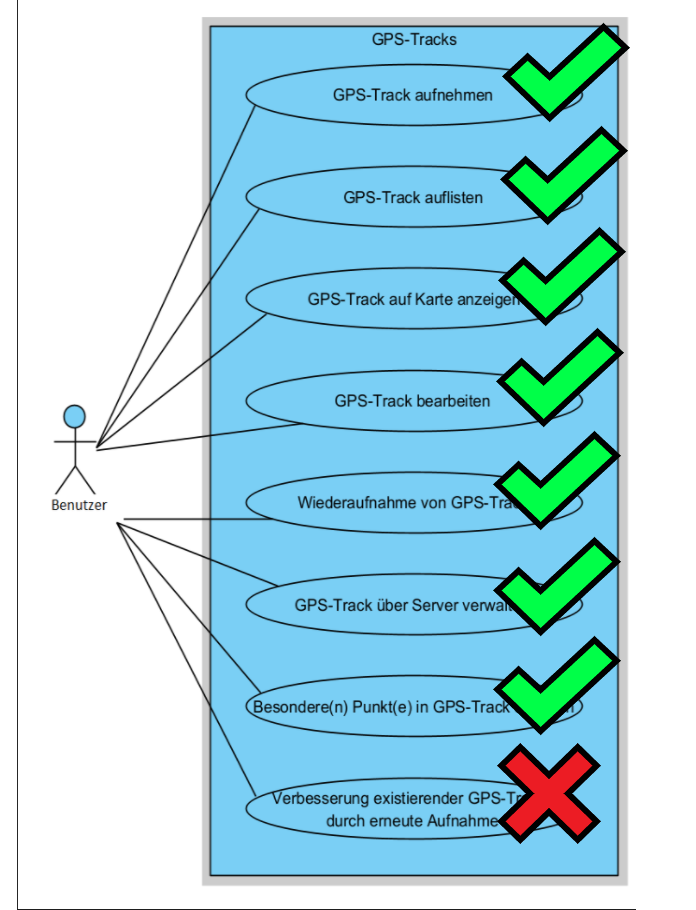
\includegraphics[scale=0.27]{use_case_comleted.png}
    \end{figure}
    Während der Entwicklung wurde auch klar, dass die Verbindung der
    Anwendung mit dem Server gesichert werden musste. Derzeit kann jeder nicht registrierte Benutzer 
    REST-Befehle verwenden, um die GPS-Dateien auf dem Server zu ändern, zu löschen oder auch auf den Server
    herunterzuladen. Das ist eine schwerwiegende Sicherheitslücke, da eine Datei mit Virencode
    an den Server gesendet werden kann und dann alle Geräte in unserem Netzwerk infiziert sein können.
    \begin{figure}[H]
        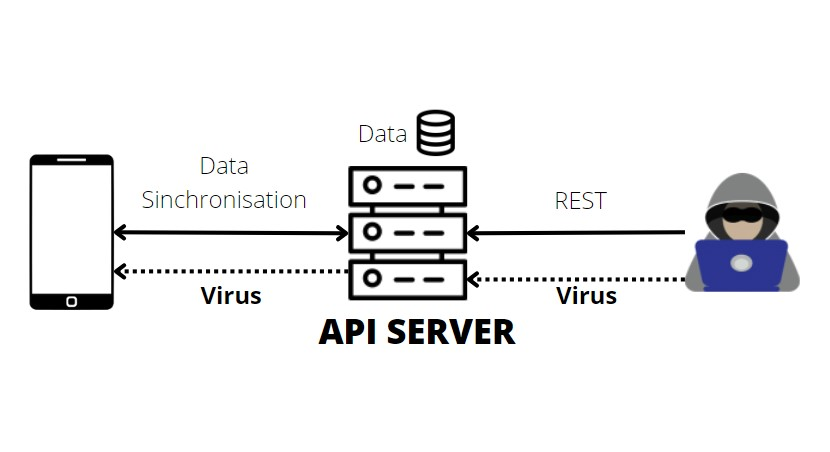
\includegraphics[scale=0.27]{virus.png}
    \end{figure}
    Aus diesem Grund sollte nächste logische Entwicklungsschritt
    daher der Authentifizierungs- und Autorisierungsprozess auf dem Server sein.
\subsection{Reflexion der Teammitglieder}
\subsubsection{Tom Nicolai}
    Ich war mit im Bereich der Programmierung der App zuständig. In den Meetings haben wir uns immer neue Features überlegt, 
    welche dann als GitHub Issues festgehalten wurden. Falls wir uns nicht während des Meetings einigen konnten, wer was macht, 
    hat sich jeder selbst das zugewiesen, worauf er grade Lust hatte. Auch haben wir unseren Zwischenstand immer mal wieder unserem 
    Auftraggeber Prof. Neugebauer gezeigt und uns Feedback dazu abgeholt. Somit konnten wir schnell sehen, ob etwas nicht so passt, 
    wie er es wollte. Die App selber haben wir in Java programmiert, was für mich gut war, da ich schon einige Erfahrung 
    in der Java Programmierung habe. Zwar habe ich noch nie eine Mobile App entwickelt, jedoch gewöhnte ich mich recht schnell 
    an die IDE und die neuen Bibliotheken. Programmiert habe ich immer nur alleine, jedoch habe ich mir auch ab und zu rat meiner 
    Teamkollegen eingeholt, bezüglich technischer Umsetzungen. Ein kleines Problem war noch, dass ich kein Android Handy besitze 
    und dementsprechend einige Features unserer App nicht ausprobieren konnte. Da wir untereinander jedoch gut vernetzt sind, 
    habe ich einfach mein neues Feature freigegeben und in unsere Gruppe geschrieben, ob es jemand testen könne. 
    Dort habe ich dann auch Feedback erhalten und konnte somit eventuelle Probleme direkt beheben. Alles in allem 
    war ich mit unserer Teamarbeit sehr zufrieden und bin mir sicher, dass wir ein gutes Produkt geschaffen haben.
\subsubsection{Aleksandr Pronin}
    Ich habe mein Team im Sommersemester kennengelernt. Zu diesem Zeitpunkt war die Android-App bereits teilweise fertig, 
    und wir mussten nur noch einen Plan für den Rest der Arbeit erstellen.
    Im ersten Schritt der Planung haben wir ein Verständnis geschaffen, wie wir die Rolle in unserem Team ungefähr verteilen können. 
    Meine Aufgabe war es, den Client-Server-Teil der Anwendung zu entwickeln und die entsprechende Dokumentation zu schreiben,
    da ich in diesem Bereich schnell und effektiv arbeiten kann.
    Das Domänenmodell, das zeigt, welche Elemente im initialen MVP vorkommen sind, wurde mir klar und ich hatte also eine gute Vorstellung
    davon, wie meine Arbeit ablaufen sollte.  Im Rahmen agile Vorgehensweisen sprachen wir ständig mit unserem Auftraggeber Prof. Neugebauer, 
    um die Anforderungen an die App zu konkretisieren und optimale Lösung konzipieren zu können. Mit all diesen Informationen konnten wir,
    technische Aspekte und Entwürfe zu User Interfaces zu erarbeiten. Wir haben außerdem beschlossen, einen wöchentlichen Daily zu führen, 
    um einen besseren Überblick über den Stand unseres Projekts zu erhalte. Ich denke, dass dies eine gute Technik ist, um im Team Gesamtergebnisse 
    zu erzielen. \\
    Bei dem Projekt, das meine Kollegen unterstütz und mitentwickelt haben, handelt es sich um eine Android-App zur 
    Speicherung von GPS-Routen und zum Austausch dieser Daten zwischen Geräten über einen Server. Application Server wurde
    in Python unter Verwendung des Flask-Frameworks geschrieben und die clientseitigen Komponenten wurden von mir 
    in Java weiterentwickelt. Rückblickend kann ich sagen, dass wir im Rahmen der Gruppenarbeit  gute Verständnis von agile 
    Entwickeln der App  und insbesondere ein kompetentes Management von dem Team besser erfassen konnten. Ich kann auch bestätigen,
    dass wir Fähigkeiten sowohl bei der Ermittlung von Anforderungen als auch bei deren Spezifizierung erworben haben und alle
    Besonderheiten der Entwicklung komplexer Softwaresysteme erkannt haben. Aus meiner Erfahrung als Werkstudent kann ich mit Zuversicht sagen,
    dass wir gemeinsam hervorragende Ergebnisse erzielt haben. Es hat Spaß gemacht, erfolgreich mit dem Team zusammenzuarbeiten und das Projekt zu 
    unterstützen. Dank meiner Kollegen(oder auch Kommilitonen) und unseres Projekts konnte ich jede Menge lernen.
\subsubsection{Alex Schechtel}
    Im zweisemestrigen Modul Software Engineering wurde ich zum ersten mal damit konfrontiert, ein erstes großes Softwareprojekt in einem Team umzusetzen.
    Größtenteils war ich im Projekt in der Implementierung der App tätig und beschäftigte mich mit dem Overlay der App und den Funktionen verschiedener Buttons.
    Ich hatte zuvor keine Erfahrung in der Appentwicklung und ko    nnte viele neue Dinge lernen.
    Dazu gehören die Gestaltung einer App und Zuweisung von Funktionen an die Buttons,
    aber auch wie man ein komplexes Softwaresystem plant und am besten umsetzt. 
    Da wir Java als Programmiersprache der App benutzten und ich schon Vorkenntnisse in Java besaß, 
    war es kein Problem sich an die Appentwicklungsumgebung zu gewöhnen.\\ 
    Ein Problem, welches ich bei der Entwicklung der App hatte, war es, den implementierten Code der Teammitglieder zu verstehen.
    Aber da wir über eine sehr gute Kommunikation verfügten, wurden diese Probleme sehr schnell aus dem Weg geschafft.
    Wenn ich mal Fragen oder Probleme bei der Entwicklung hatte wurde mir von den Teamkollegen immer geholfen.
    In den Meetings (im Team) herschte immer ein sehr lockeres und angenehmes Arbeitsklima, 
    was zusätzlich zu einer guten Gruppenarbeit beigetragen hat. \\
    Die Kommunikation mit dem Themensteller bereitete uns auch keine Probleme. Es konnte immer nach Anfrage ein Termin gefunden werden. 
    Alles in allem hat mir das Projekt viel Spaß gemacht, da ich jede Menge neue Dinge lernen konnte und ich denke, 
    dass wir gute Arbeit geleistet haben.
\subsubsection{Quang Duy Pham}
	Vor dem Besuch des Moduls Software Engineering hatte ich keine Erfahrung mit der Arbeit im Team oder in einem komplexen Projekt. Dies war eine große Herausforderung für mich zu meistern.Am Anfang habe ich mich für Tester und Analyse entschieden. Als Analyse habe ich einige Ideen zu Use-Cases und Struktur des Projekts gegeben, aber es gab keinen signifikanten Beitrag in Rolle Analyse und hauptsächlich noch als a Tester.\par
	Obwohl ich den Quellcode nicht direkt implementiert habe, da mir die Programmiererfahrung fehlt. Ich muss immer noch den Quellcode und die Projektstruktur verstehen, um erfolgreiche Testfälle durchzuführen. Als Tester habe ich viel über Testmethoden und Dokumentationenbeschreibung gelernt. Außerdem habe ich einige kleine Beiträge gemacht, die nicht codierungsbezogen sind, wie Format der Dokumentationen prüfen, Mehrsprachenfunktion implementieren und kleine UI anpassen.\par
	Ich konnte Fehler jedoch nicht selbst beheben, weil ich Angst habe, dem Code kaputt zu machen, also bat ich oft andere Teamkollegen um Hilfe.\par
	Nach dem Modul Software Engineering hoffe ich, dass ich meine Kommunikation mit anderen verbessern konnte. Ich würde gerne mehr über das Programmieren lernen und beim nächsten Mal als Implementierung arbeiten. Schließlich möchte ich bessere Sprachkenntnisse haben, um bessere Dokumentationen schreiben zu können.\par
\end{document}
